\documentclass[aspectratio=43]{beamer}
\usepackage{pgfplots}
\usepackage{tikz} 
\usetikzlibrary{patterns}


% Define Colors
\definecolor{customcolor}{RGB}{100,65,5}
\definecolor{pgfbackgroundcolor}{RGB}{245,225,185}
\definecolor{pgfnodecolor}{RGB}{55,40,30}

% Theme settings
\usetheme{Madrid}
\usecolortheme[named=customcolor]{structure}
\pgfplotsset{compat=1.17}

% Information
\title{Redesign Assignment}
\author{Luis Kraker}
\institute{FH JOANNEUM}
\date{Technical Documentation}

\begin{document}

% Title Frame
\begin{frame}
  \titlepage
\end{frame}

% Frame discussing bad graph points
\begin{frame}
\frametitle{Bad Design}
\begin{columns}[T] % Align columns at the top
\begin{column}{.48\textwidth}
   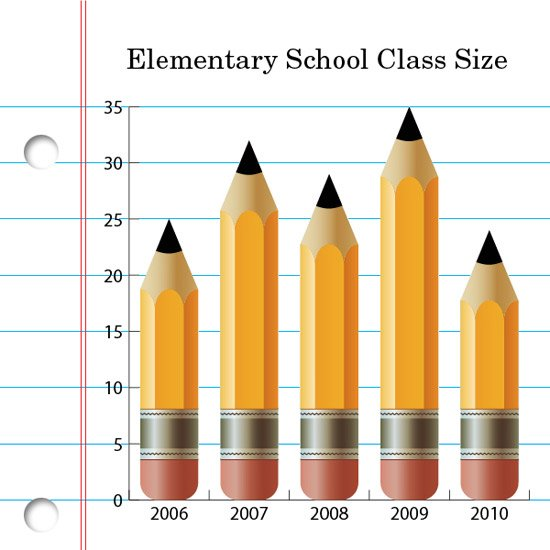
\includegraphics[width=\linewidth]{bad_graph.jpg}
\end{column}
\begin{column}{.48\textwidth}
    \begin{itemize}
        \item Pencil images distort data perception.
        \item Difficult to determine precise values.
        \item Overuse of different colors.
        \item Inappropriate choice of pencil form for graph bars.
        \item No specification of units on y-axis and x-axis.
    \end{itemize}
\end{column}
\end{columns}
\end{frame}


% Frame on how to improve the graph
\begin{frame}
    \frametitle{Improvement Strategies}
        \begin{itemize}
            \item Use simple bars for accurate data representation.
            \item Incorporate a grid to improve visual clarity.
            \item Add a descriptive title to the graph.
            \item Minimize color variance by using a consistent color palette instead .
            \item Make the graph visually appealing without distorting the data.
            \item Clearly label the x- and y-axis with units.
        \end{itemize}
    \end{frame}

% Frame on how to improve the graph
\begin{frame}
    \frametitle{New Design}
    \centering
    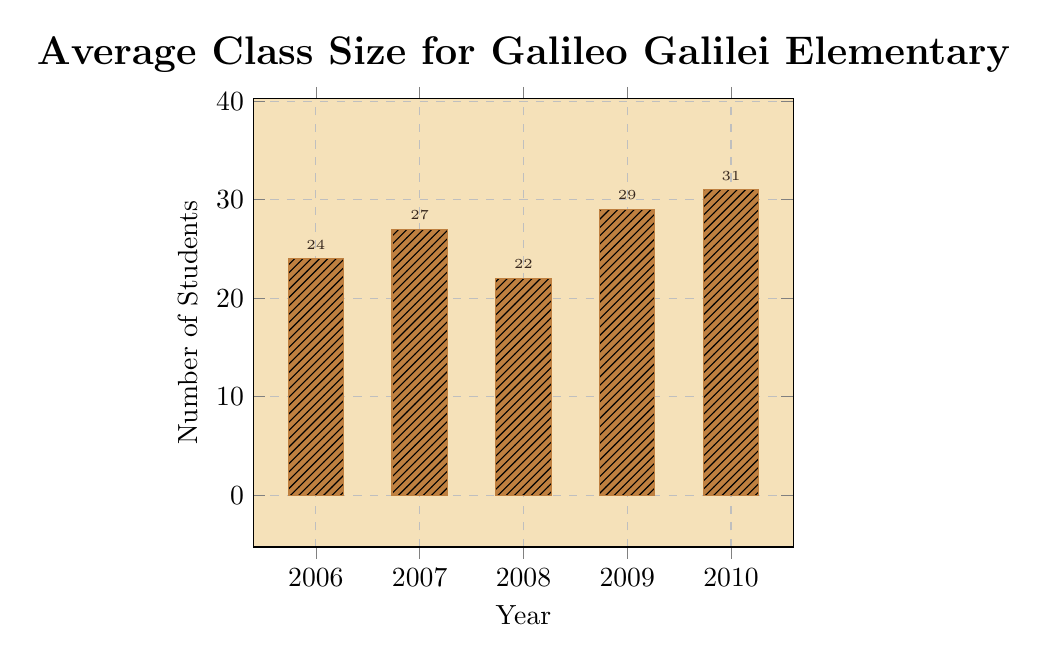
\begin{tikzpicture}
    \begin{axis}[
        ybar, % Bar graph
        bar width=20pt, % Width of the bars
        title={Average Class Size for Galileo Galilei Elementary}, % Main title
        title style={align=center, font=\Large\bfseries}, % Center the title if it wraps
        enlargelimits=0.15,
        ylabel={Number of Students}, % Label for the y-axis
        xlabel={Year}, % Label for the x-axis
        symbolic x coords={2006, 2007, 2008, 2009, 2010},
        xtick=data,
        nodes near coords, % Display data value near bars
        nodes near coords align={vertical},
        % apply color to noes near cords
        every node near coord/.append style={font=\tiny, color=pgfnodecolor},
        ymin=0, ymax=35, % Adjusted for better fit of the annotation
        xmajorgrids=true,
        ymajorgrids=true,
        grid style=dashed,
        axis background/.style={fill=pgfbackgroundcolor}, % Background color for the plot area
        ]
    
    \addplot +[
        postaction={
            pattern=north east lines
        },
        fill=brown, % Softer brown color
        draw=brown,
        ] coordinates {(2006,24) (2007,27) (2008,22) (2009,29) (2010,31)};
    
    \end{axis}
    \end{tikzpicture}

\end{frame}
    
    

\end{document}
